\chapter{Metodología}
\label{chap:metodologia}

\section{Diseño general del estudio}
\label{sec:diseno}

El estudio tiene carácter empírico y aplicado. Parte de datos de mercado, construye una variable objetivo financiera mediante inversión de Black-76, entrena modelos de regresión y evalúa tanto rendimiento predictivo como coherencia explicativa. La Figura~\ref{fig:metodologia-general} resume el flujo metodológico. La ampliación de trazabilidad estructural del ETL se recoge en el apéndice \ref{app:data-structures} y la de ingeniería de desarrollo y despliegue en el apéndice \ref{app:workflow-dev}.

\begin{figure}[htbp]
\centering
\small
\begin{tikzpicture}[node distance=8mm and 7mm]
  \node[data] (raw) {Datos fuente};
  \node[process, right=of raw] (etl) {ETL y validaciones};
  \node[data, right=of etl] (iv) {VOLATILITY\_DB};
  \node[process, below=of iv] (feat) {Feature engineering};
  \node[process, left=of feat] (split) {Splits temporales};
  \node[process, left=of split] (search) {K-folds e hiperparámetros};
  \node[process, below=of search] (retrain) {Reentrenamiento};
  \node[service, right=of retrain] (pkg) {Paquete dashboard};
  \node[service, right=of pkg] (deploy) {API, dashboard y cloud};
  \draw[arrow] (raw) -- (etl);
  \draw[arrow] (etl) -- (iv);
  \draw[arrow] (iv) -- (feat);
  \draw[arrow] (feat) -- (split);
  \draw[arrow] (split) -- (search);
  \draw[arrow] (search) -- (retrain);
  \draw[arrow] (retrain) -- (pkg);
  \draw[arrow] (pkg) -- (deploy);
\end{tikzpicture}
\caption{Flujo metodológico del proyecto.}
\label{fig:metodologia-general}
\end{figure}

El flujo no es lineal sólo en apariencia. Cada bloque deja salidas persistidas y comprobables que sirven de entrada al siguiente, de modo que la metodología puede auditarse por etapas. Primero se consolida la base financiera; después se fija un espacio de variables coherente con la superficie; a continuación se comparan familias bajo un protocolo temporal común; y, por último, se transforma el modelo seleccionado en un sistema consultable. Este diseño responde a cuatro principios metodológicos.

\begin{itemize}
  \item \textbf{Separación de responsabilidades:} ETL, modelización, explicabilidad y servicio no se mezclan en un único bloque opaco.
  \item \textbf{Trazabilidad de extremo a extremo:} cada predicción puede rastrearse hasta datos, configuración y versión de modelo.
  \item \textbf{Comparabilidad entre familias:} todas las alternativas compiten bajo las mismas reglas de split, métricas y reentrenamiento.
  \item \textbf{Lectura profesional del resultado:} el producto final no es sólo una tabla de métricas, sino un modelo interpretable y servible.
\end{itemize}

Esta estructura es importante porque condiciona la credibilidad de los resultados. Si el entrenamiento fuese correcto pero las explicaciones o el servicio no reutilizasen exactamente la misma lógica de features, la calidad del sistema quedaría comprometida aunque las métricas numéricas fueran buenas.

\section{Datos y muestra analizada}
\label{sec:datos}

El pipeline de datos transforma ficheros de contratos, operaciones y tipos en una base final de volatilidad implícita. Hay tres fuentes principales: 
\begin{itemize}
    \item \textbf{Contratos}: aportan información de código, strike y vencimiento.
    \item \textbf{Operaciones}: aportan precio, cantidad, hora y contrato.
    \item \textbf{Series de EONIA/\texteuro{}STR}: permiten calcular el tipo compuesto aplicable hasta vencimiento.
\end{itemize}


\begin{wrapfigure}{r}{0.48\textwidth}
\vspace{-1em}
\centering

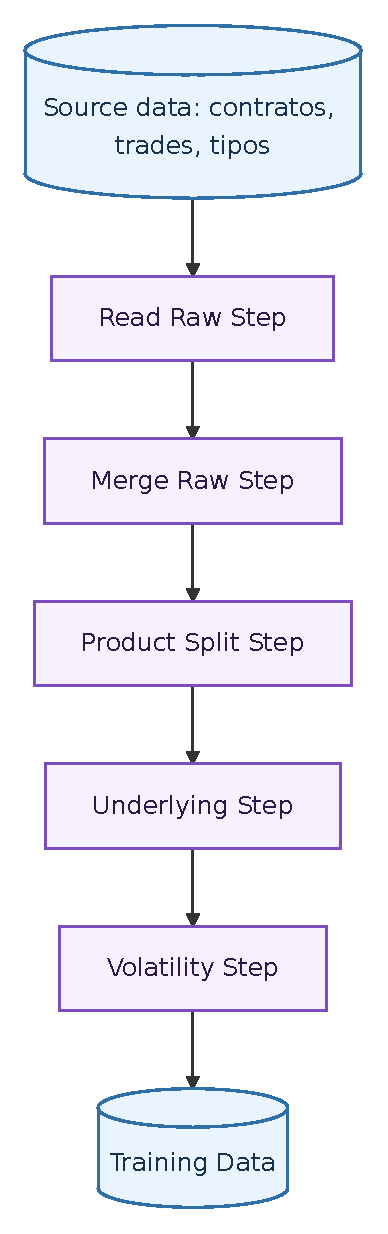
\includegraphics[
    width=\linewidth,
    height=0.32\textheight,
    keepaspectratio
]{../doc/mermaid-pdf/index/02.pdf}
\caption{Secuencia principal de procesado de datos.}
\label{fig:doc-index-2}

\end{wrapfigure}

En el cálculo de tipos se asume una aproximación operativa: no se dispone de un calendario TARGET2 explícito dentro del pipeline, por lo que el conteo de días hábiles se implementa con \texttt{pd.bdate\_range} (días laborables estándar). La composición se aplica exactamente como en el código: se recorre cada día hábil del intervalo, se toma \(r_i\) (retrocediendo al último dato disponible si ese día no existe en la serie) y se multiplica
\(1 + r_i n_i / 360\), con \(n_i=3\) cuando el día hábil es lunes y \(n_i=1\) en el resto. Después se anualiza como
$$\left(\prod_i\left(1+\frac{r_i n_i}{360}\right)-1\right)\cdot \frac{360}{d_c}.$$

La guía de referencia para la lógica de tipos compuestos es la del BCE para \texteuro{}STR:
\url{https://www.ecb.europa.eu/stats/euro-short-term-rates/interest_rate_benchmarks/WG_euro_risk-free_rates/shared/pdf/ecb.Compounded_euro_short-term_rate_calculation_rules.en.pdf}. En esta memoria se documenta de forma explícita que la implementación actual reproduce la convención descrita en el código (incluido el peso 3 en lunes) y debe interpretarse como aproximación operativa mientras no se incorpore un calendario TARGET2 completo en la construcción de \texttt{Rate}.



\vspace{0.8em}
\begin{wrapfigure}{r}{0.48\textwidth}

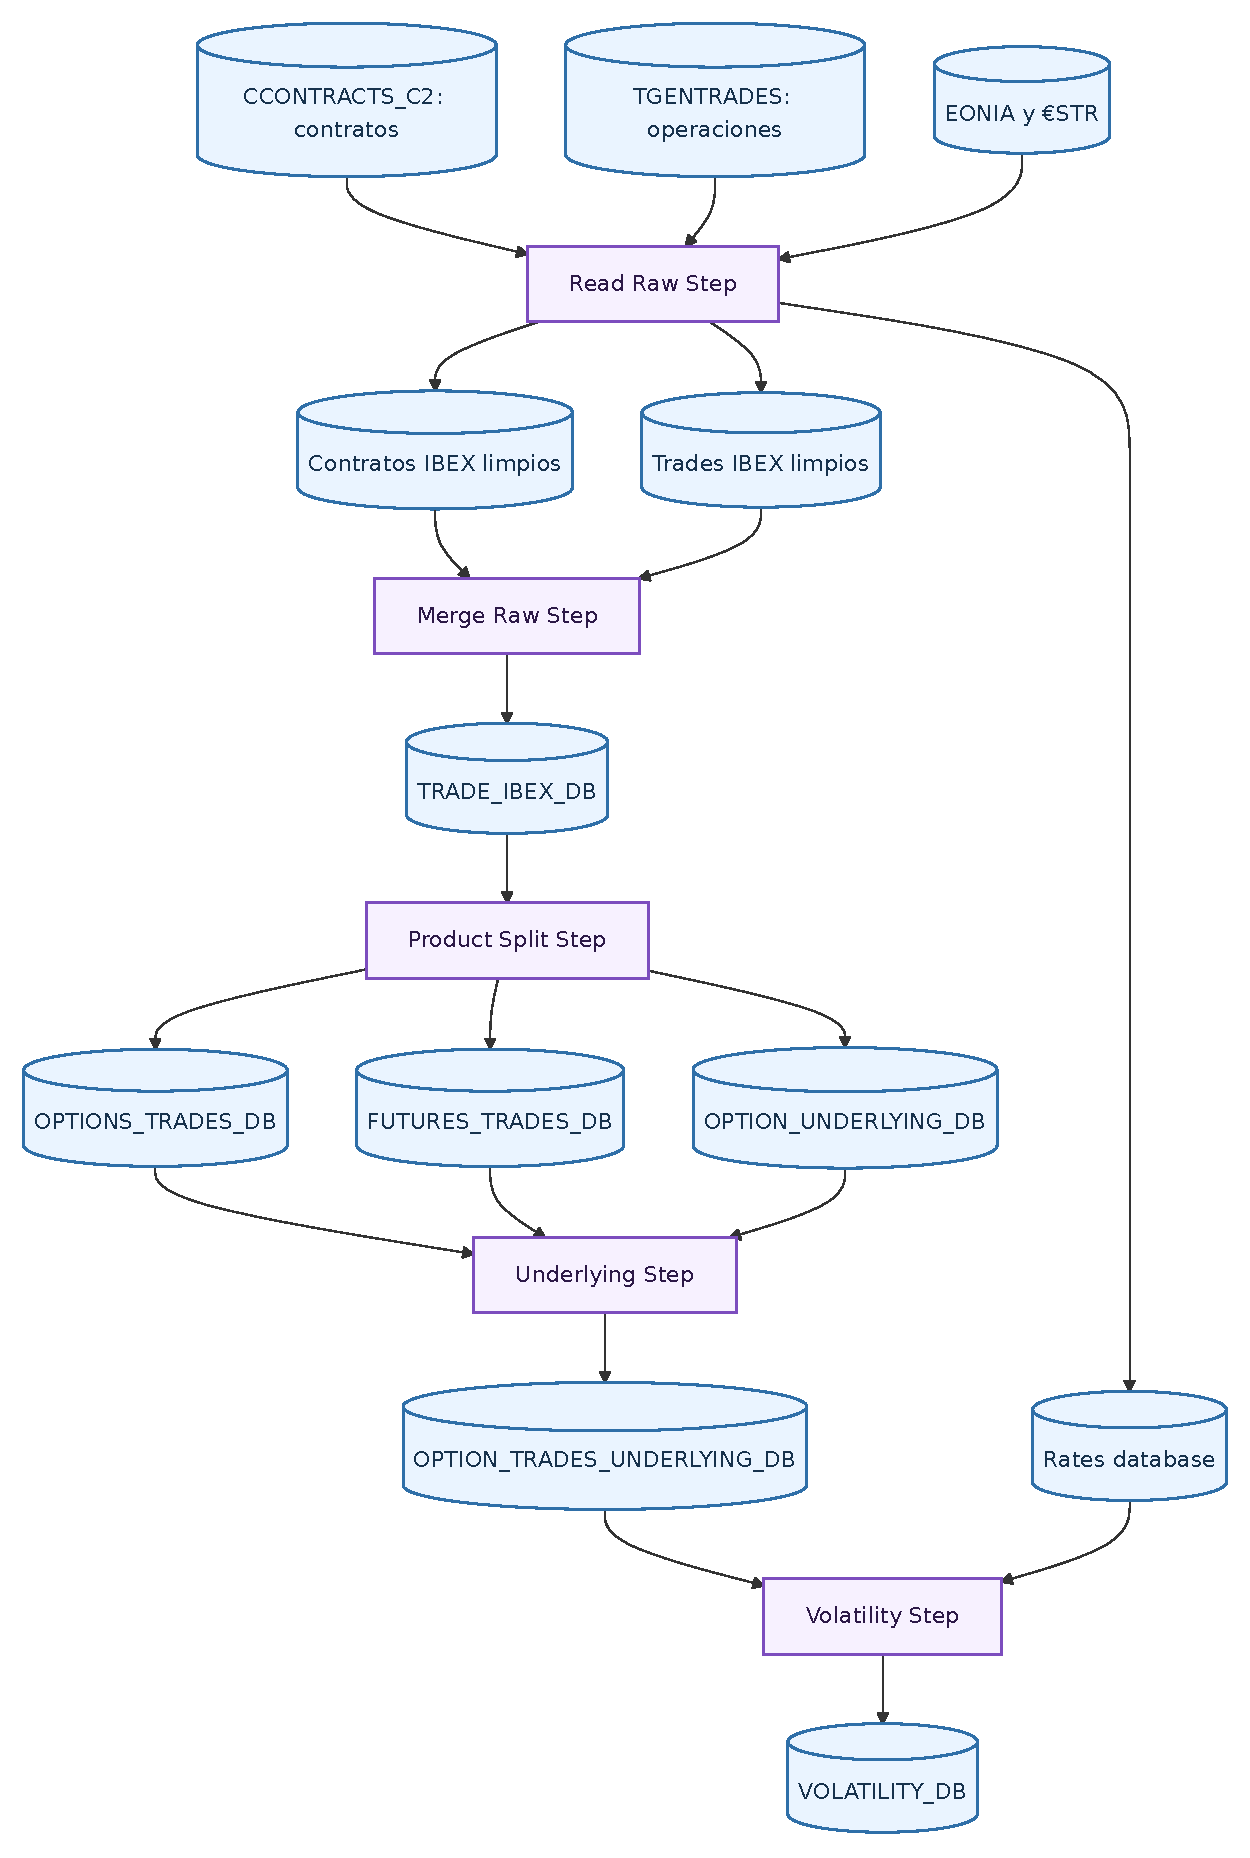
\includegraphics[
    width=\linewidth,
    height=0.32\textheight,
    keepaspectratio
]{../doc/mermaid-pdf/data/index/01.pdf}
\caption{Pipeline completo de datos hasta VOLATILITY\_DB.}
\label{fig:doc-data-index-1-small}

\vspace{-1em}
\end{wrapfigure}





La cadena ETL se materializa por pasos, como muestran las
Figuras~\ref{fig:doc-index-2} y~\ref{fig:doc-data-index-1-small}.
Esta organización permite cachear salidas intermedias, validar contratos
de datos y aislar responsabilidades: los \emph{StepLoaders} orquestan
lectura, cache y validación, mientras que los \emph{builders} construyen
la salida material de cada paso.

La Figura~\ref{fig:loaders-builders-schema} resume esta separación entre clases \emph{loader} y clases \emph{builder}. El detalle extenso de las estructuras de datos que va produciendo cada etapa se recoge además en el apéndice \ref{app:data-structures}, para no sobrecargar el cuerpo principal con un diagrama demasiado largo.

\begin{wrapfigure}{l}{0.48\textwidth}
\centering
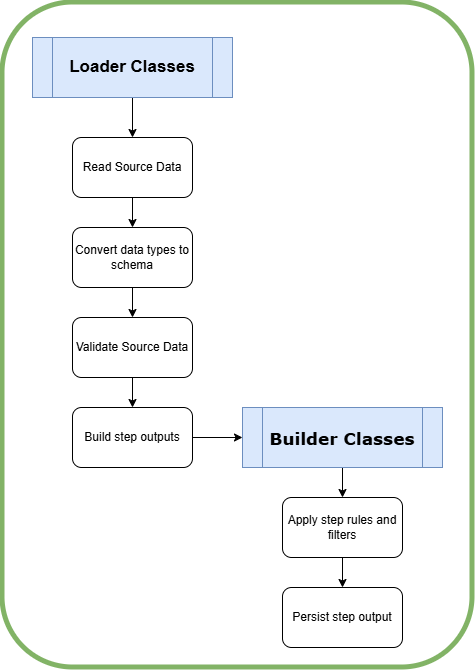
\includegraphics[
    width=\linewidth,
    height=0.32\textheight,
    keepaspectratio
]{../imgs/loaders_builders_schema.drawio.png}
\caption{\small Esquema de responsabilidades entre \emph{loaders} y \emph{builders} en el ETL.}
\label{fig:loaders-builders-schema}
\end{wrapfigure}



Los datos se filtran al dominio de opciones IBEX mensuales y futuros mensuales asociados. Las opciones semanales y contratos fuera de dominio se excluyen para mantener coherencia contractual.

La salida final contiene fecha y hora de ejecución, código de opción, tipo call/put, precio negociado, strike, futuro subyacente, precio del subyacente, desfase temporal opción-subyacente (minutos), tiempo a vencimiento, tipo compuesto y volatilidad implícita.

El \textbf{primer paso}, \texttt{Read Raw Step}, normaliza ficheros de mercado con o sin cabecera, elimina columnas auxiliares no pertenecientes al esquema final, convierte fechas, horas y numéricos, filtra prefijos IBEX y construye una serie homogénea de tipos. La base de tipos combina EONIA ajustado por el spread configurado antes de la fecha de corte y \texteuro{}STR desde esa fecha.  Figuras~\ref{fig:doc-data-raw-read-1}, \ref{fig:doc-data-raw-read-2}.


\par
\clearpage




\begin{figure}[htp]
\centering

\begin{subfigure}[t]{0.48\textwidth}
    \centering
    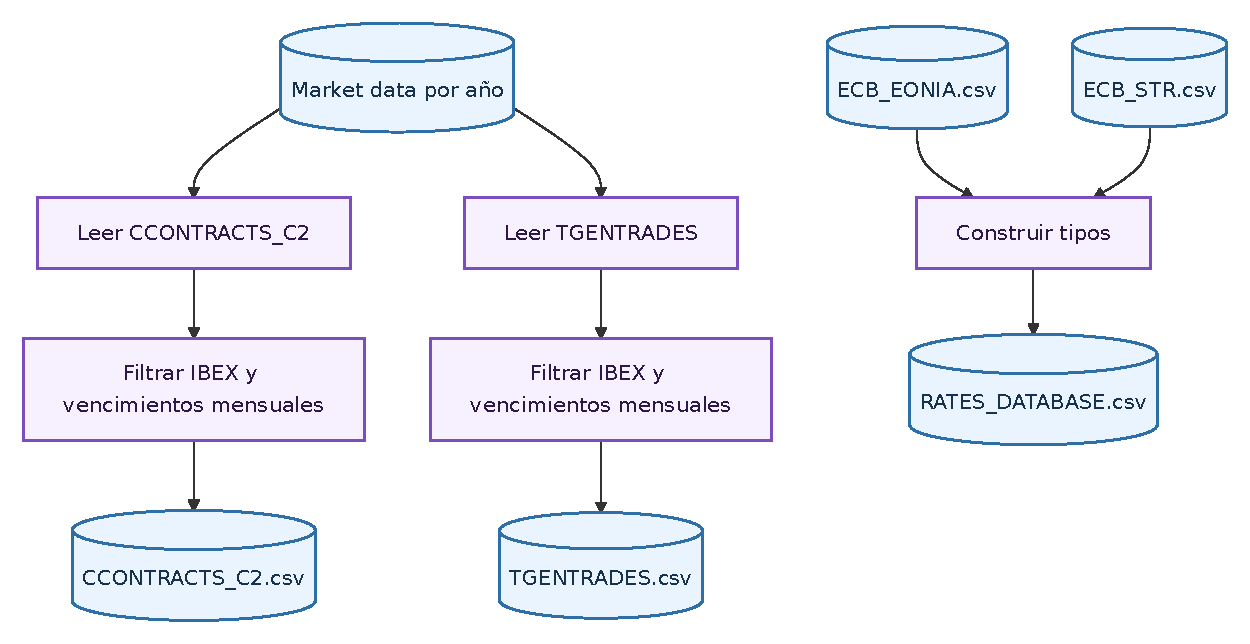
\includegraphics[width=\linewidth]{../doc/mermaid-pdf/data/raw-read/01.pdf}
    \caption{\small Paso 1. Lectura y normalización de datos.}
    \label{fig:doc-data-raw-read-1}
\end{subfigure}
\hfill
\begin{subfigure}[t]{0.48\textwidth}
    \centering
    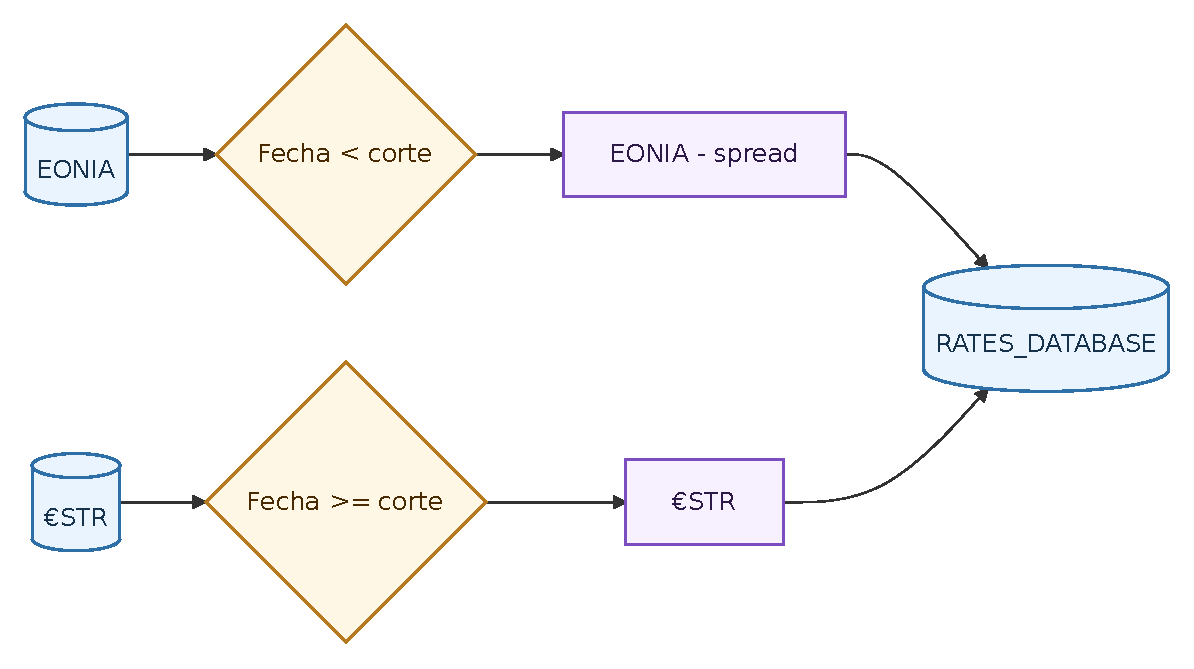
\includegraphics[width=\linewidth]{../doc/mermaid-pdf/data/raw-read/02.pdf}
    \caption{\small Paso 1. Construcción de tipos.}
    \label{fig:doc-data-raw-read-2}
\end{subfigure}
\label{fig:doc-data-raw-read}
\end{figure}



\begin{figure}[!htbp]
\centering
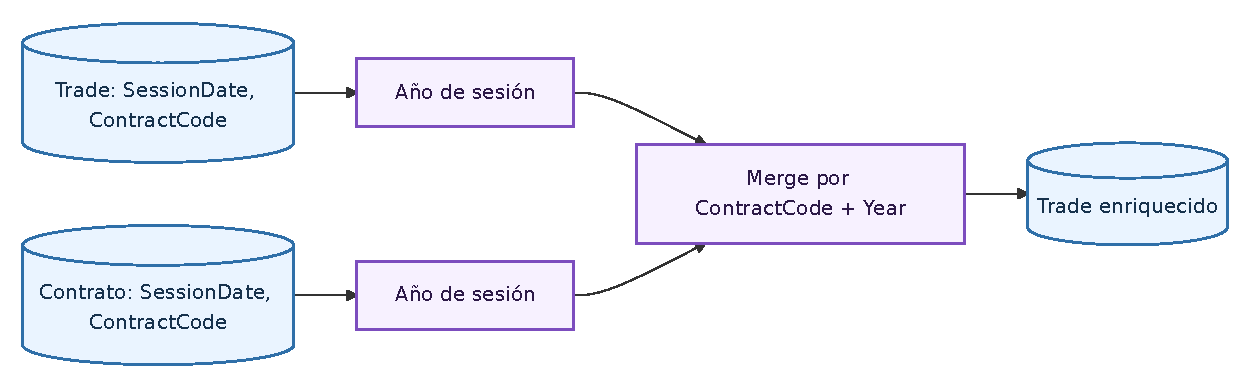
\includegraphics[
    width=0.6\linewidth,
    height=0.32\textheight,
    keepaspectratio
]{../doc/mermaid-pdf/data/merge-raw/02.pdf}
\caption{\small Paso 2. Unión por código de contrato y año de sesión.}
\label{fig:doc-data-merge-raw-2}
\end{figure}


El \textbf{segundo paso}, \texttt{Merge Raw Step}, une operaciones y contratos por \texttt{ContractCode} y año de sesión, imputa vencimientos con la regla del tercer viernes e imputa strikes desde el tramo configurado del código cuando la fuente no lo trae completo. Las Figuras~\ref{fig:doc-data-merge-raw-1} y~\ref{fig:doc-data-merge-raw-2} resumen visualmente esta fase.


\begin{figure}[!htbp]
\centering

\begin{subfigure}[t]{0.48\textwidth}
    \centering
    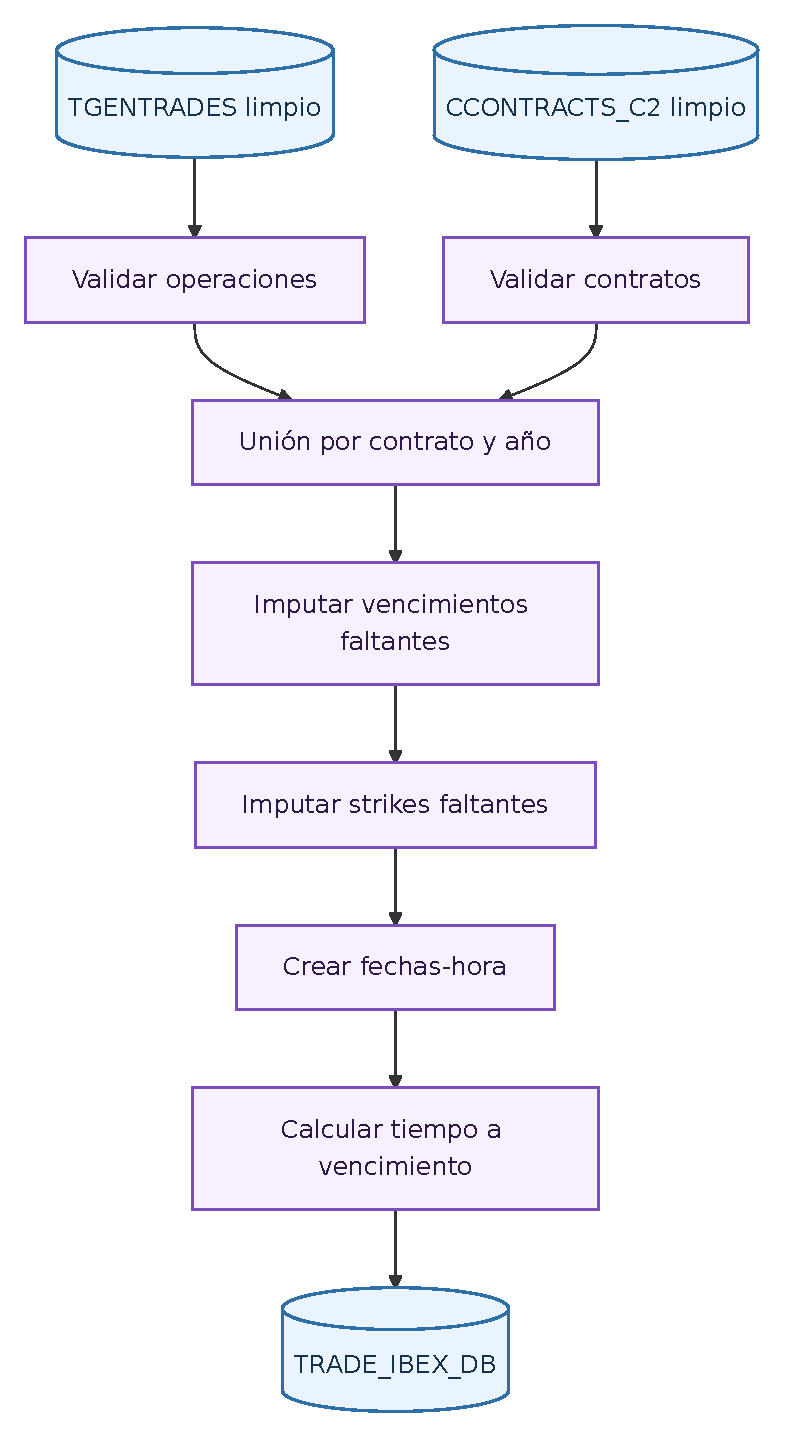
\includegraphics[width=0.6\linewidth]{../doc/mermaid-pdf/data/merge-raw/01.pdf}
    \caption{\small Paso 2. Unión de operaciones con información contractual.}
    \label{fig:doc-data-merge-raw-1}
\end{subfigure}
\hfill
\begin{subfigure}[t]{0.48\textwidth}
    \centering
    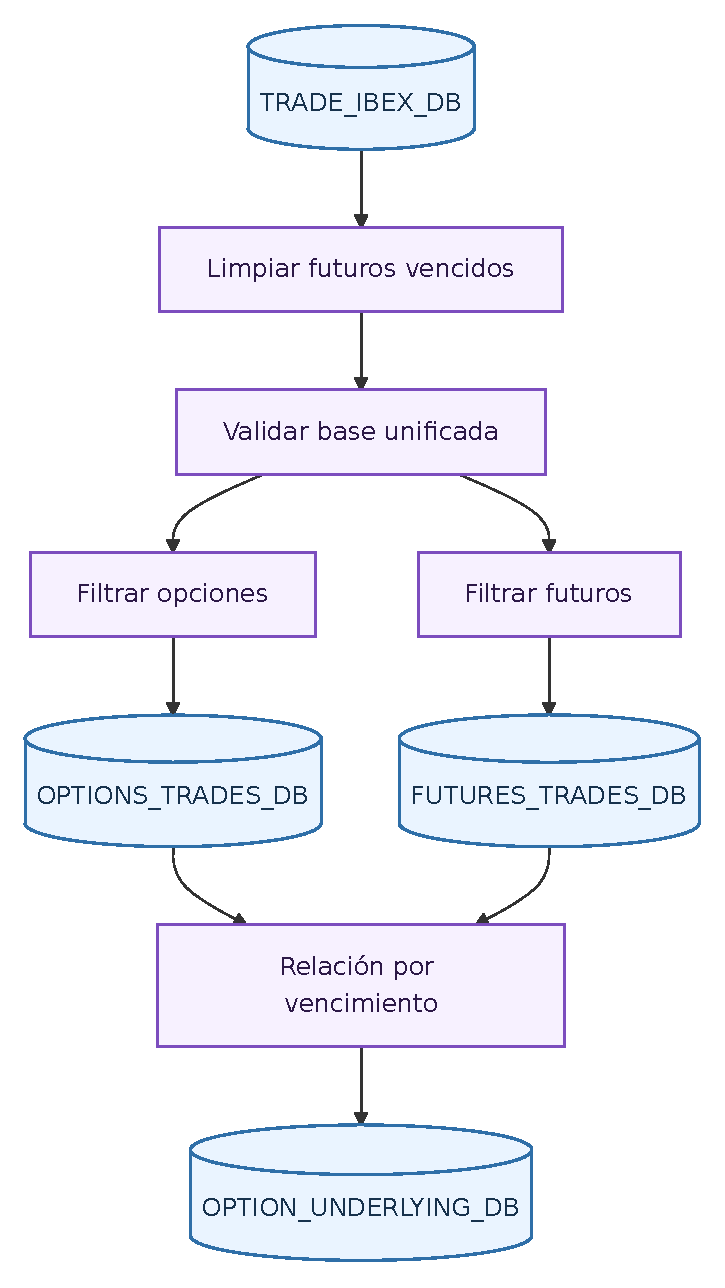
\includegraphics[width=0.6\linewidth]{../doc/mermaid-pdf/data/product-split/01.pdf}
    \caption{\small Paso 3. Separación de operaciones por producto.}
    \label{fig:doc-data-product-split-1}
\end{subfigure}

\caption{\small Unión de datos contractuales y separación por producto.}
\label{fig:doc-data-raw-read-and-split}
\end{figure}


El \textbf{tercer paso}, \texttt{Product Split Step}, divide la base unificada en opciones, futuros y relación opción-futuro por vencimiento. 

\textbf{El cuarto}, \texttt{Underlying Step}, garantiza el emparejamiento temporal sin lookahead y resuelve el precio de futuro subyacente mediante una unión temporal \emph{as-of}: para cada opción selecciona el último trade del futuro con instante de ejecución menor o igual al de la opción. Esta decisión evita lookahead dentro del propio ETL. 



\begin{figure}[htp]
\centering
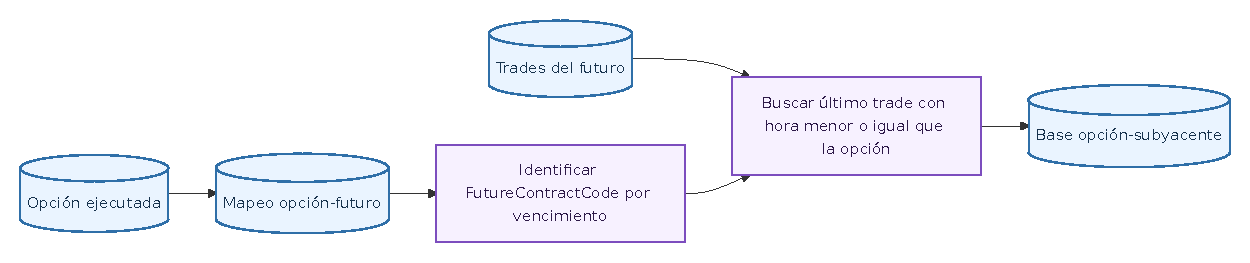
\includegraphics[
    width=0.8\linewidth,
    height=0.32\textheight,
    keepaspectratio
]{../doc/mermaid-pdf/data/underlying/01.pdf}
\caption{\small Paso 4. Asignación de futuro subyacente a cada opcion.}
\label{fig:doc-data-underlying-1}
\end{figure}



\textbf{El quinto}, \texttt{Volatility Step}, filtra operaciones sin subyacente fiable o con desfase temporal excesivo, calcula el tipo compuesto hasta vencimiento y resuelve la volatilidad implícita por Black-76 inverso (Figuras~\ref{fig:doc-data-volatility-1} y~\ref{fig:doc-data-volatility-2}).




\begin{figure}[htp]
\centering
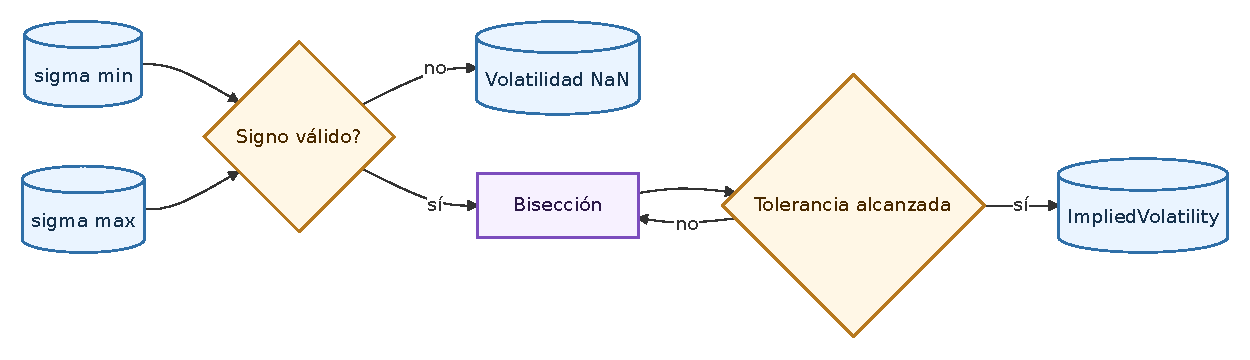
\includegraphics[
    width=0.8\linewidth,
    height=0.32\textheight,
    keepaspectratio
]{../doc/mermaid-pdf/data/volatility/02.pdf}
\caption{\small Paso 5. Solver por bisección de la volatilidad implícita.}
\label{fig:doc-data-volatility-2}
\end{figure}





En este \textbf{último paso} se aplican reglas de calidad relevantes para evitar sesgos en entrenamiento: se excluyen filas sin subyacente válido, filas con desfase opción-subyacente superior al umbral configurado de 180 minutos, y filas cuya volatilidad implícita no puede resolverse de forma válida (por ejemplo, sin cambio de signo del solver o con soluciones no finitas). Estas decisiones son coherentes con el análisis exploratorio y con las validaciones financieras del pipeline.


\begin{figure}[htp]
\centering
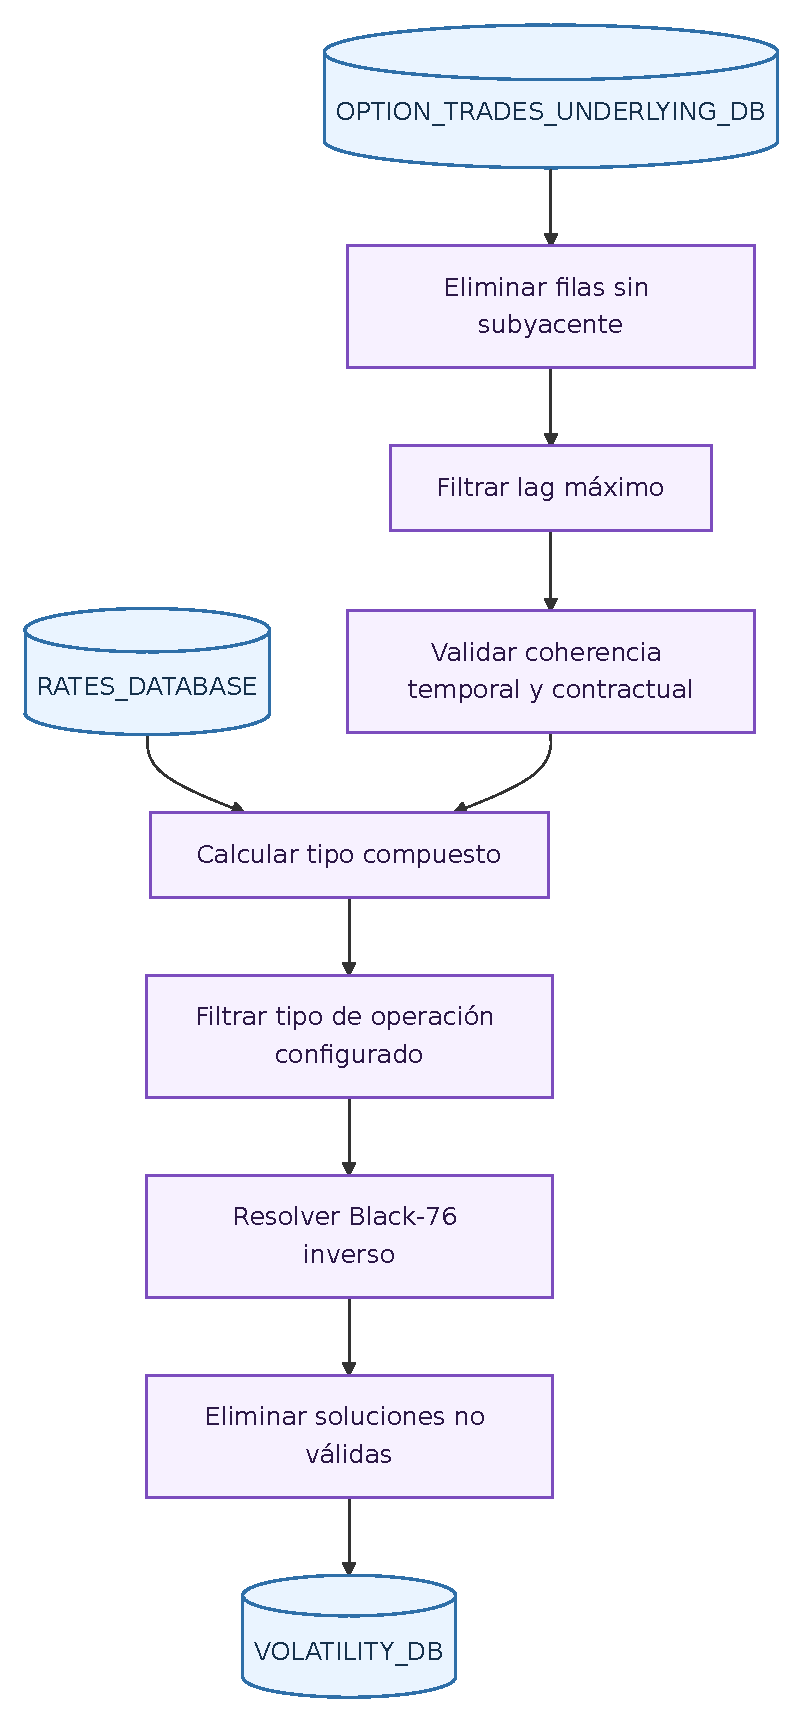
\includegraphics[
    width=0.5\linewidth,
    keepaspectratio
]{../doc/mermaid-pdf/data/volatility/01.pdf}
\caption{\small Paso 5. Cálculo de volatilidad implícita.}
\label{fig:doc-data-volatility-1}
\end{figure}



\newpage



\section{Validaciones y tratamiento financiero}
\label{sec:validaciones-datos}

El ETL aplica validaciones transversales: precios positivos, cantidades positivas, ausencia de claves duplicadas, control de missing values, vencimientos coherentes, strikes compatibles con el código de contrato y subyacente temporalmente anterior a la operación de la opción. Esta última condición es crítica para evitar utilizar información futura.

Para evitar ambigüedades, en esta memoria se distinguen dos conceptos de lag: el desfase opción-subyacente del ETL (en minutos) y el lag temporal del split de entrenamiento (en número de fechas) usado más adelante en la validación de modelos.

El cálculo de volatilidad implícita se realiza en el último paso. Se eliminan operaciones sin subyacente fiable, se calcula el tipo compuesto hasta vencimiento y se resuelve la ecuación \eqref{eq:iv-inversion}. Si no existe cambio de signo en el intervalo de búsqueda o la solución es no finita, la observación se marca como no resoluble y no alimenta el entrenamiento. La Figura~\ref{fig:doc-data-index-2} resume estas validaciones sobre el contrato y su interpretación.

\begin{figure}[h]
\centering
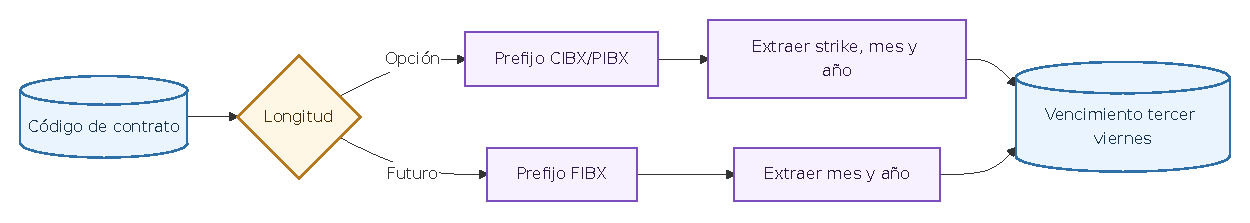
\includegraphics[width=0.85\textwidth,height=0.40\textheight,keepaspectratio]{../doc/mermaid-pdf/data/index/02.pdf}%
\caption{\small Validacion e interpretacion del codigo de contrato.}
\label{fig:doc-data-index-2}
\end{figure}

\section{Variables y feature engineering}
\label{sec:variables}

Las entradas raw visibles son \texttt{OptionType}, \texttt{StrikePrice}, \texttt{UnderlyingPrice}, \texttt{TimeToExpiration} y \texttt{Rate}. Estas variables son suficientes para reconstruir el vector de entrenamiento y también son comprensibles para un usuario financiero que consulte la API.

No se aplica una fase de selección de variables ex post (ni filtros automáticos de descarte por importancia) porque el foco metodológico es simular una operación directa con un conjunto de entradas financieras estable, reproducible y utilizable tal cual en API/dashboard. La comparación entre familias se hace, por diseño, sobre el mismo espacio de variables para aislar el efecto de la arquitectura y no de una poda específica de features.

El vector transformado se diseña para representar la geometría de la superficie. La Tabla~\ref{tab:features} resume las variables derivadas.

\begin{table}[htbp]
\centering
\small
\begin{tabular}{lll}
\toprule
Feature & Fórmula & Motivo \\
\midrule
\texttt{TTEYears} & \(T=T_{\mathrm{dias}}/365\) & Vencimiento en años \\
\texttt{sqrtTTEYears} & \(\sqrt{T}\) & Escala temporal de Black-76 \\
\texttt{logMoneyness} & \(\log(F/K)\) & Posición relativa frente al strike \\
\texttt{logMoneynessSq} & \(\log(F/K)^2\) & Curvatura del smile \\
\texttt{logMoneynessXSqrtTTE} & \(\log(F/K)\sqrt{T}\) & Interacción smile-vencimiento \\
\texttt{logForwardMoneyness} & \(\log(Fe^{rT}/K)\) & Ajuste por tipo y vencimiento \\
\texttt{rate} & \(r\) & Sensibilidad directa a tipos \\
\texttt{isCall}, \texttt{isPut} & Indicadores & Tipo de opción \\
\bottomrule
\end{tabular}
\caption{Features financieras utilizadas por los modelos.}
\label{tab:features}
\end{table}

Esta elección evita que el modelo dependa de niveles absolutos de strike que pueden cambiar con el régimen de mercado. El moneyness permite comparar contratos negociados en momentos distintos del IBEX, mientras que el vencimiento y sus transformaciones capturan estructura temporal. Las Figuras~\ref{fig:doc-models-features-1-small} y~\ref{fig:doc-models-features-2-small} muestran la construcción y motivación financiera de estas variables.


\begin{figure}[!htbp]
\centering
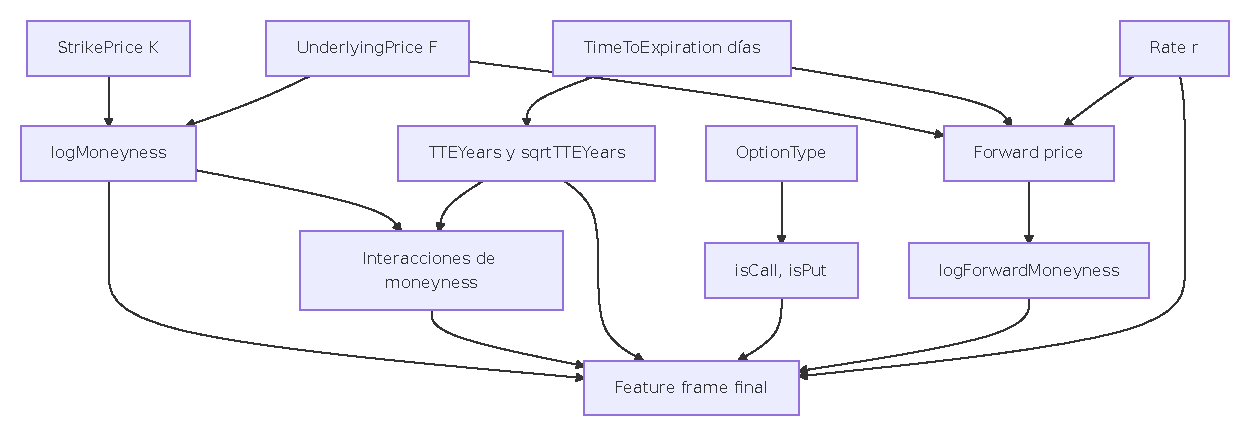
\includegraphics[width=0.8\linewidth]{../doc/mermaid-pdf/models/features/01.pdf}
\caption{\small Construccion de features financieras.}
\label{fig:doc-models-features-1-small}
\end{figure}

\begin{figure}[!htbp]
\centering
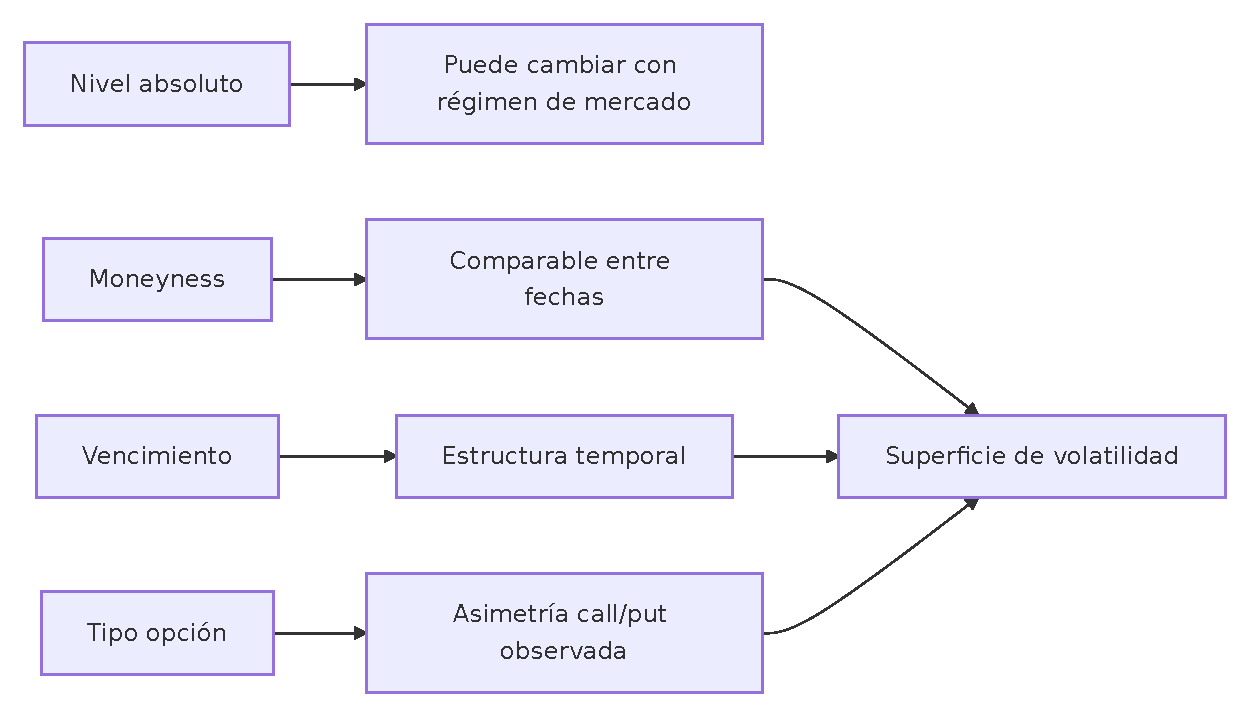
\includegraphics[width=0.6\linewidth]{../doc/mermaid-pdf/models/features/02.pdf}
\caption{\small Motivacion financiera de las features.}
\label{fig:doc-models-features-2-small}
\end{figure}




\section{Familias de modelos}
\label{sec:familias}

El repositorio implementa una abstracción común para familias de modelos. Cada familia declara nombre, parámetros fijos, espacio de búsqueda, instanciación, entrenamiento y persistencia. La Tabla~\ref{tab:familias} resume su papel en el estudio.

\begin{table}[htbp]
\centering
\small
\begin{tabular}{p{0.25\textwidth}p{0.62\textwidth}}
\toprule
Familia & Papel metodológico \\
\midrule
Regresión lineal & Baseline interpretable para evaluar cuánto aporta la no linealidad. \\
Random Forest & Modelo tabular robusto ante interacciones y no linealidades sin escalado. \\
XGBoost & Boosting regularizado con early stopping interno y alta capacidad predictiva. \\
Red neuronal secuencial & Aproximador flexible con escalado de variables numéricas y early stopping sobre validación interna. \\
Quantum Inspired NN & Variante clásica de red neuronal con estructura tensorial inspirada en ideas cuánticas; se evalúa como arquitectura implementada, no como computación cuántica física. \\
\bottomrule
\end{tabular}
\caption{Familias de modelos entrenadas en el proyecto.}
\label{tab:familias}
\end{table}

Todas las familias heredan una interfaz común: declaran parámetros fijos, espacio de búsqueda, instanciación, entrenamiento, persistencia y número de configuraciones exploradas. Esta homogeneidad permite comparar un baseline lineal, modelos de árboles, boosting y arquitecturas neuronales con el mismo protocolo de selección. En la familia Quantum Inspired, el cálculo sigue siendo clásico: las features se proyectan a un embedding, se reordenan como tensor y se contraen mediante una capa tensor-train antes de una capa densa final. El concepto y su implementación práctica se detallan en el apéndice \ref{app:quantum-inspired}.

La elección de familias responde a una lógica comparativa.

\begin{itemize}
  \item La \textbf{regresión lineal} fija una referencia interpretable y permite medir cuánto valor añade la no linealidad una vez creadas las features correctas.
  \item \textbf{Random Forest} y \textbf{XGBoost} representan dos formas distintas de explotar interacciones tabulares complejas sin exigir el mismo tipo de preprocesado que las redes.
  \item Las \textbf{redes neuronales} sirven para comprobar si una arquitectura más flexible mejora realmente el problema o sólo incrementa el coste y la complejidad de explicación.
  \item La variante \textbf{Quantum Inspired} introduce una hipótesis arquitectónica diferenciada manteniendo computación clásica, lo que permite valorar su aportación real frente a alternativas más estándar.
\end{itemize}

La interfaz común del repositorio hace además que la comparación sea metodológicamente limpia. Todas las familias pasan por los mismos splits temporales, las mismas métricas y el mismo proceso de reentrenamiento y conversión a paquete de dashboard. Eso evita que una familia ``gane'' por haber sido evaluada con un protocolo distinto del resto.



\section{Splits temporales y selección}
\label{sec:validacion}

\begin{figure}[!htbp]
\centering
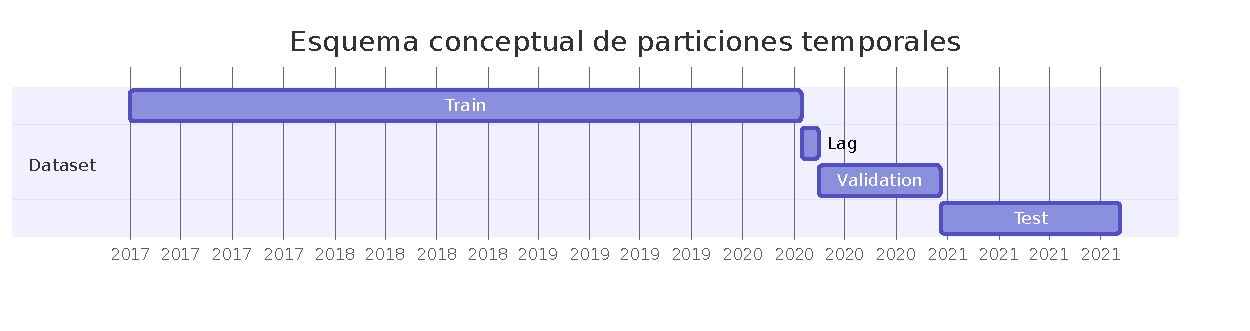
\includegraphics[width=0.85\textwidth,height=0.40\textheight,keepaspectratio]{../doc/mermaid-pdf/models/splits-kfolds/01.pdf}%
    \caption{\small Esquema conceptual de particiones temporales.}
    \label{fig:doc-models-splits-kfolds-1-small}
\end{figure}

La validación sigue tres principios. 
\begin{enumerate}
    \item Respeto del orden temporal: train precede a validation y test.
    \item Puede existir un lag de fechas entre bloques para reducir contaminación temporal.
    \item Exclusividad de contratos: si el mismo contrato aparece en más de un split, se conserva en un único bloque según volumetría y prioridad.
\end{enumerate} 





\begin{wrapfigure}{r}{0.48\textwidth}
\centering
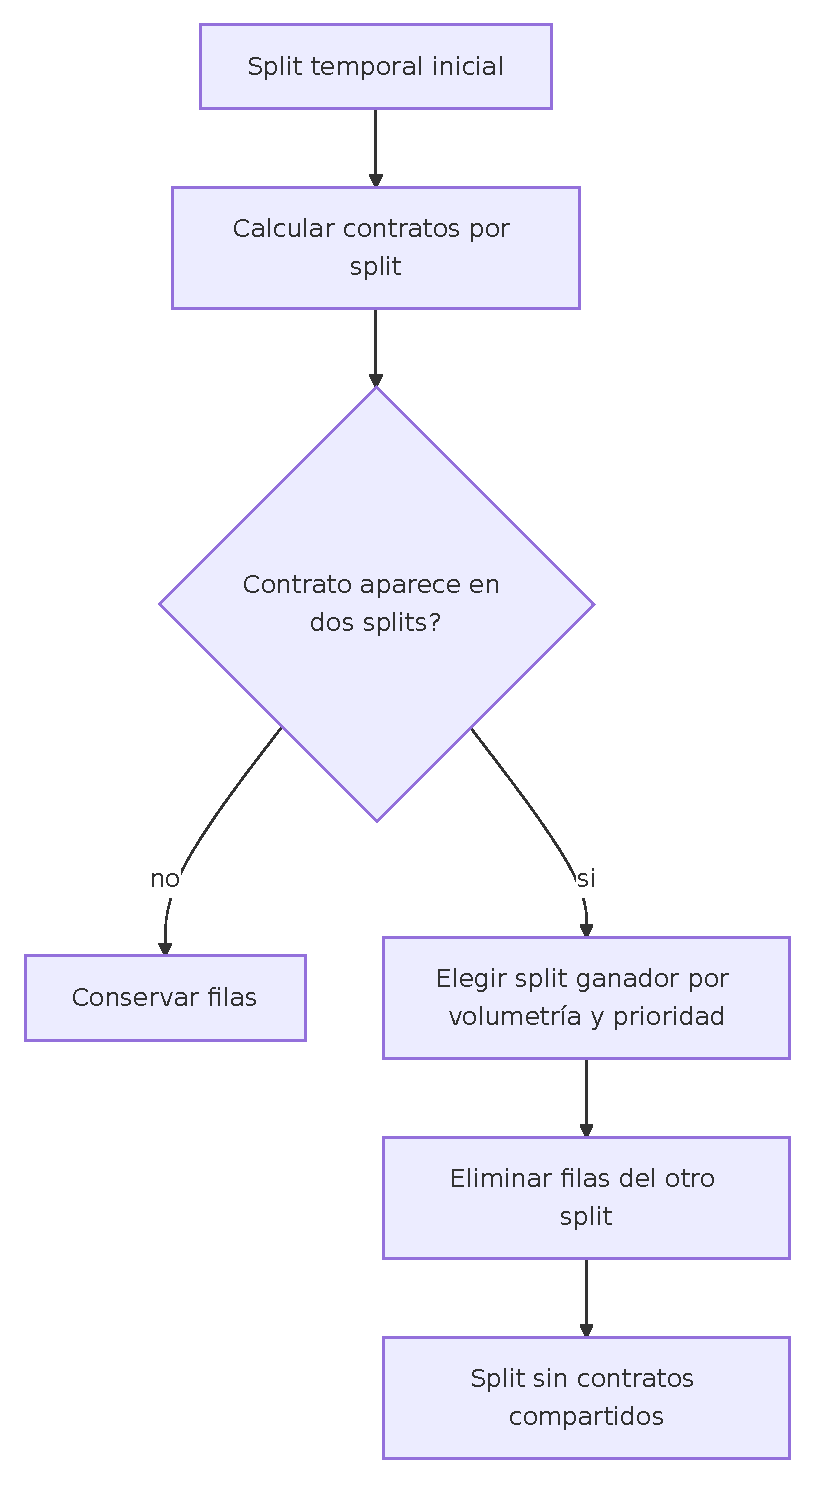
\includegraphics[
    width=\linewidth,
    height=0.32\textheight,
    keepaspectratio
]{../doc/mermaid-pdf/models/splits-kfolds/02.pdf}
    \caption{\small Control de contratos compartidos entre splits.}
    \label{fig:doc-models-splits-kfolds-2-small}
\end{wrapfigure}



Esta última regla es relevante porque una opción puede negociarse durante varios días. Si un contrato aparece en entrenamiento y validación, el modelo podría aprender rasgos idiosincráticos del contrato y ofrecer una estimación optimista. Las Figuras \ref{fig:doc-models-index-2}, \ref{fig:doc-models-splits-kfolds-1-small}, \ref{fig:doc-models-splits-kfolds-2-small} y~\ref{fig:doc-models-splits-kfolds-3} resumen la lógica temporal, la separación con lag y el control de contratos compartidos.


La búsqueda de hiperparámetros se realiza con k-folds temporales. Estos k-folds se construyen exclusivamente dentro del bloque de entrenamiento, de modo que validation y test externos quedan fuera del proceso de búsqueda. Para cada candidato se calculan MAE, RMSE y \(R^2\) en train y validation. 

\par
\clearpage

La selección usa una métrica compuesta:



\begin{equation}
CE_1 = RMSE_{val}+\alpha \cdot std(RMSE_{val})+\beta \cdot \max(0, RMSE_{val}-RMSE_{train}).
\label{eq:ce1}
\end{equation}

Esta métrica penaliza error de validación, inestabilidad entre folds y gap de sobreajuste. Según la configuración del repositorio, \(\alpha=0.25\) y \(\beta=0.75\).


\begin{figure}[h]
\centering
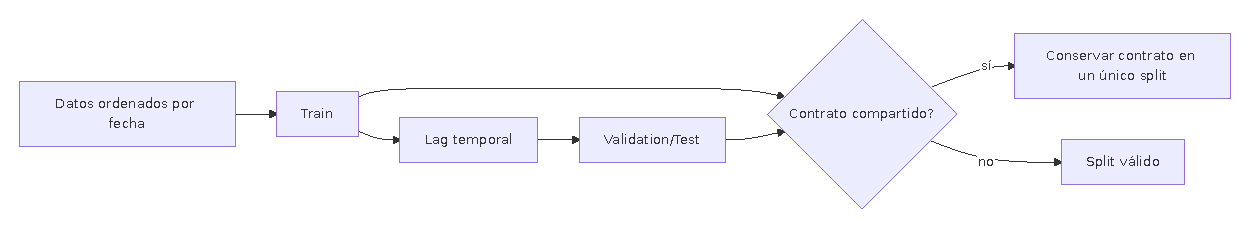
\includegraphics[width=\textwidth,height=0.35\textheight,keepaspectratio]{../doc/mermaid-pdf/models/index/02.pdf}%
\caption{\small Control temporal y exclusividad de contratos.}
\label{fig:doc-models-index-2}
\end{figure}


\begin{figure}[h]
\centering
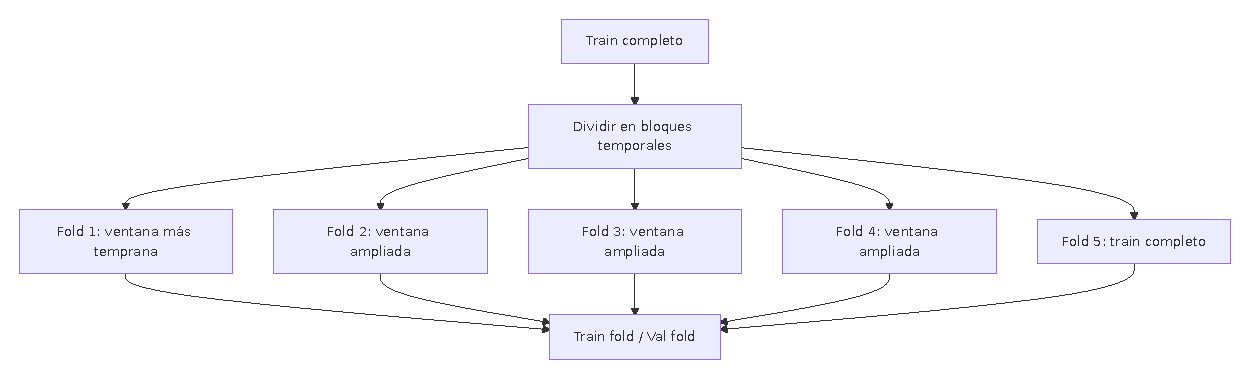
\includegraphics[width=0.85\textwidth,height=0.40\textheight,keepaspectratio]{../doc/mermaid-pdf/models/splits-kfolds/03.pdf}%
\caption{\small Construccion de k-folds temporales.}
\label{fig:doc-models-splits-kfolds-3}
\end{figure}




\vspace{-0.3cm}
\section{Reentrenamiento y progressive ATM}
\label{sec:progressive-main}

\begin{figure}[h]
\centering
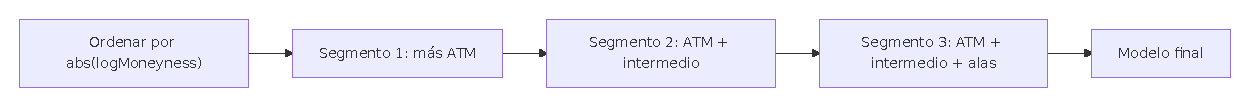
\includegraphics[width=\textwidth,height=0.35\textheight,keepaspectratio]{../doc/mermaid-pdf/models/retraining-progressive/02.pdf}%
\caption{\small Entrenamiento progressive ATM por segmentos.}
\label{fig:doc-models-retraining-progressive-2}
\end{figure}

Después de seleccionar hiperparámetros, el modelo se reentrena en dos fases: train/validation y final test. En la fase final se ajusta con trainval y se evalúa contra test. La métrica de reentrenamiento incorpora el rendimiento observado en selección:

\begin{equation}
CE_2 = RMSE_{val}+\gamma \cdot CE_1+\beta \cdot \max(0, RMSE_{val}-RMSE_{train}),
\label{eq:ce2}
\end{equation}

con \(\gamma=0.25\) y \(\beta=0.75\) en la configuración actual.

Es importante precisar que \(CE_2\) se utiliza para monitorizar consistencia en la fase train/validation. La evaluación definitiva de generalización del modelo se realiza siempre sobre el bloque test fuera de muestra.

El proyecto incluye una variante progressive ATM. Ordena observaciones por \(|\log(F/K)|\), de más cercano al ATM a más alejado, y divide el entrenamiento en segmentos. La idea financiera es aprender primero la zona central, habitualmente más líquida y estable, y después incorporar zonas más alejadas. En modelos no iterativos se implementa mediante pesos; en XGBoost y redes se implementa mediante fases acumulativas. Por su carácter experimental, esta variante se menciona aquí y se desarrolla en el apéndice \ref{app:progressive}. Las Figuras~\ref{fig:doc-models-retraining-progressive-1} y~\ref{fig:doc-models-retraining-progressive-2} muestran el reentrenamiento del mejor candidato y los segmentos ATM.




\begin{figure}[h]
\centering
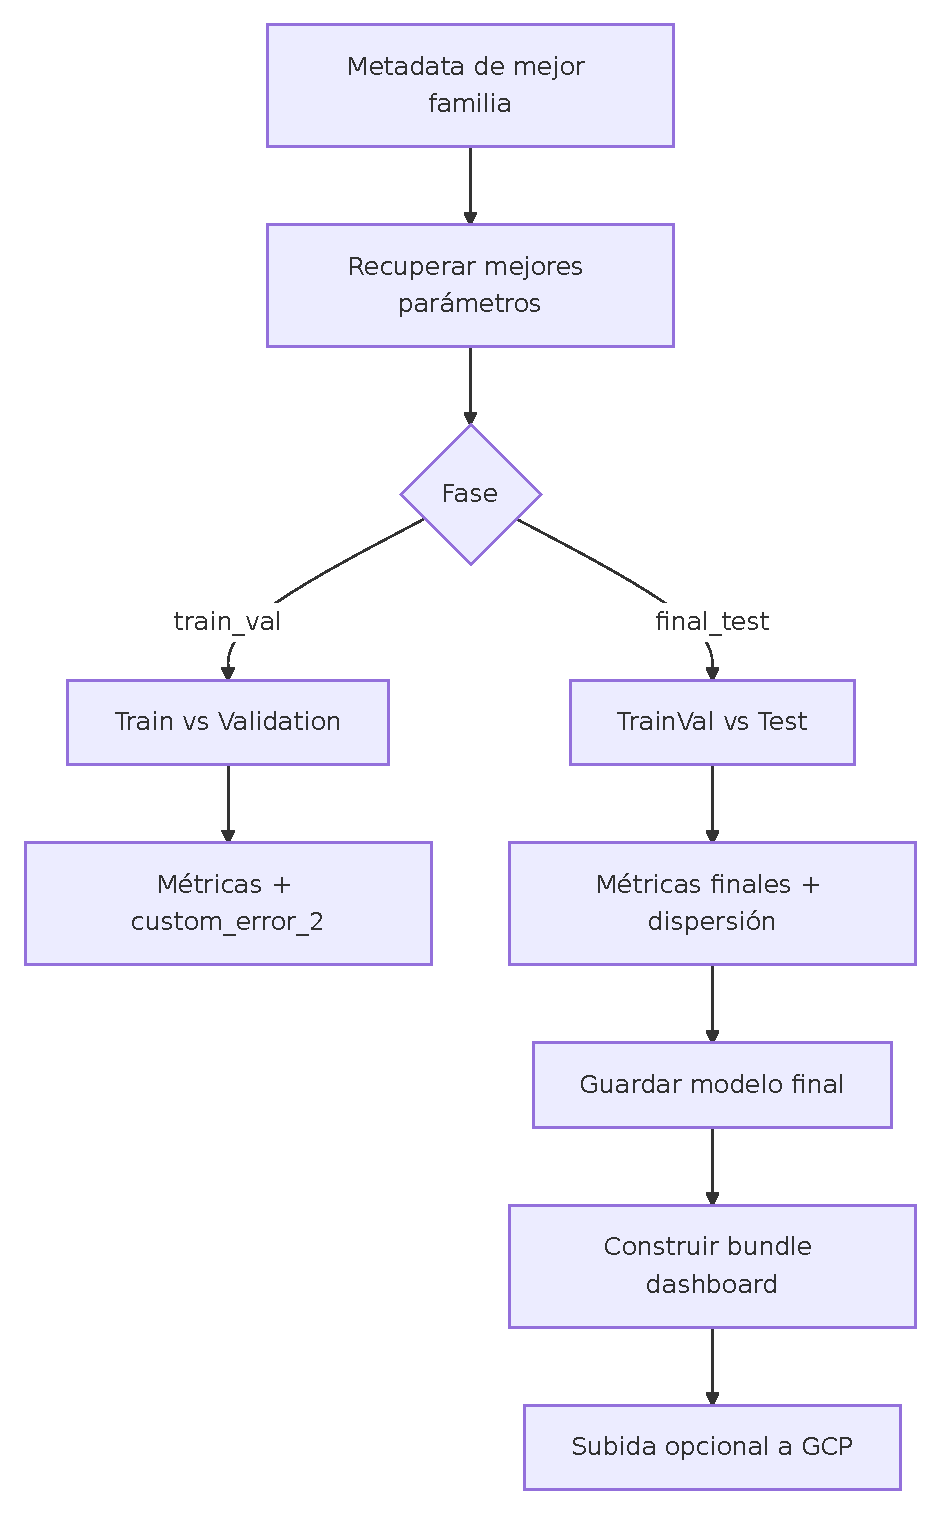
\includegraphics[width=0.6\textwidth]{../doc/mermaid-pdf/models/retraining-progressive/01.pdf}%
\caption{\small Reentrenamiento del mejor candidato.}
\label{fig:doc-models-retraining-progressive-1}
\end{figure}


\newpage

\section{Construcción del dashboard}
\label{sec:dashboard-metodo}

El dashboard no entrena modelos. Consume paquetes autocontenidos generados desde modelos finales (ver Figura ~\ref{fig:doc-dashboard-model-to-dashboard-1}). Cada paquete contiene dataset con predicciones, residuales y error absoluto, muestras para explicabilidad local, puntos de referencia de superficies, SHAP global y local, árboles surrogate, regresor simbólico, vecinos, superficies, ICE, ALE y diagnóstico agregado. La base teórica y operativa de SHAP, ALE y regresión simbólica se desarrolla respectivamente en los apéndice \ref{app:shap}, apéndice \ref{app:ale} y apéndice \ref{app:symbolic-regression}.

\begin{figure}[h]
    \centering
    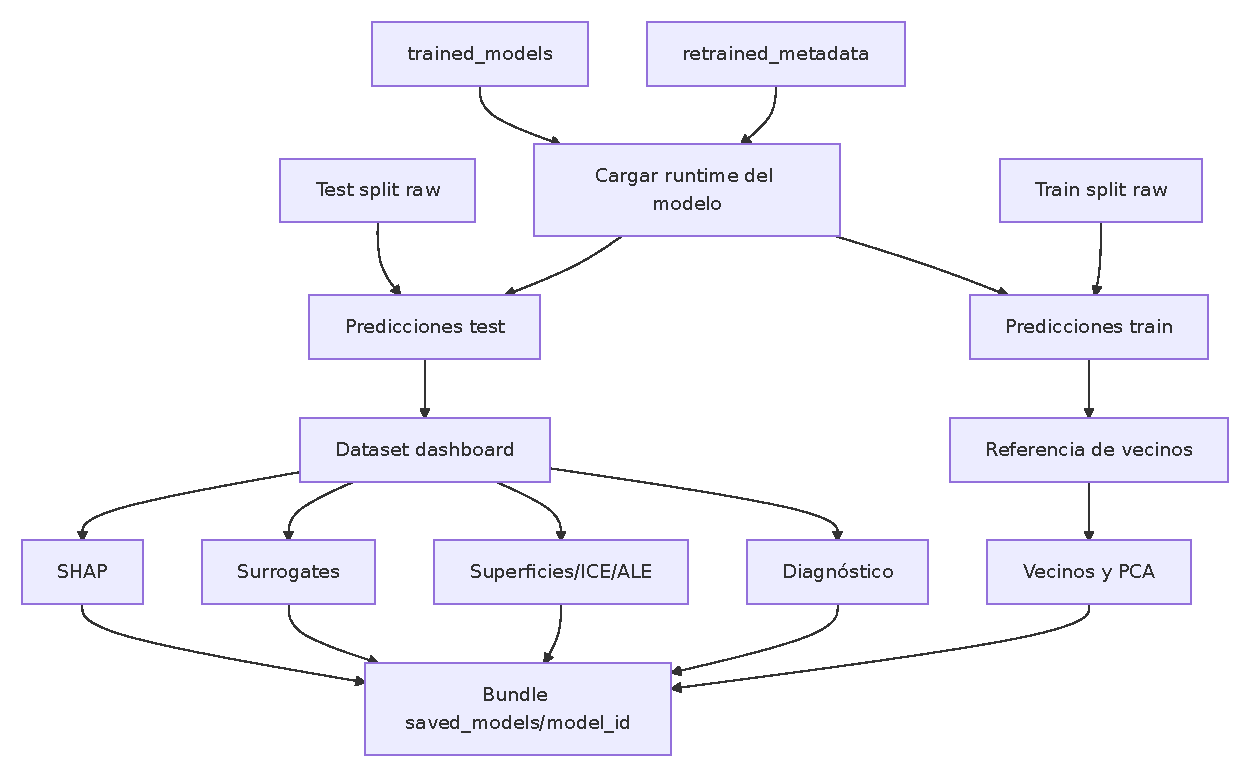
\includegraphics[width=0.85\textwidth,height=0.40\textheight,keepaspectratio]{../doc/mermaid-pdf/dashboard/model-to-dashboard/01.pdf}%
    \caption{\small Conversión de modelo final a paquete visualizable.}
    \label{fig:doc-dashboard-model-to-dashboard-1}
\end{figure}

La transformación de un modelo final a este paquete no modifica el predictor: carga el runtime, aplica el mismo feature engineering sobre train y test, calcula artefactos explicativos y persiste una carpeta autocontenida en \texttt{src/dashboard/saved\_models/}.

La aplicación se estructura en cuatro pestañas, resumidas en la Tabla~\ref{tab:dashboard-tabs}. Esta organización responde a preguntas distintas y evita confundir error predictivo con explicación.

En particular, la lectura SHAP se divide en dos niveles complementarios: \textbf{SHAP global} en la pestaña \emph{Global Explainability} (drivers y patrones agregados) y \textbf{SHAP local} en la pestaña \emph{Sample Explainability}, donde se muestra el \emph{Local SHAP Waterfall} para justificar una predicción concreta. La formalización de ambas lecturas se recoge en el apéndice \ref{app:shap}.

\begin{table}[htbp]
\centering
\small
\begin{tabular}{p{0.30\textwidth}p{0.58\textwidth}}
\toprule
Pestaña & Pregunta principal \\
\midrule
Behaviour And Surface & ¿Cómo responde el modelo ante cambios de moneyness, vencimiento y otras variables financieras? \\
Global Explainability & ¿Qué variables y patrones dominan las predicciones globales? \\
Sample Explainability & ¿Por qué una muestra concreta recibe esa volatilidad y tiene soporte histórico? \\
Diagnosis & ¿Dónde acierta y dónde falla el modelo en la superficie? \\
\bottomrule
\end{tabular}
\caption{Pestañas del dashboard y función analítica.}
\label{tab:dashboard-tabs}
\end{table}



Las vistas del dashboard son necesarias para localizar dónde aparece esa compresón. El scatter \emph{predicted vs actual} debe confirmar si los extremos altos y bajos se acercan a la media; el residual heatmap debe separar error por moneyness y vencimiento; y las cajas \emph{Error by Moneyness} y \emph{Error by Maturity} deben indicar si los extremos de moneyness o los vencimientos cortos concentran el fallo.

Las Figuras~\ref{fig:doc-dashboard-behaviour-surface-1}, \ref{fig:doc-dashboard-diagnosis-1}, \ref{fig:doc-dashboard-global-explainability-1}, \ref{fig:doc-dashboard-sample-explainability-1} y~\ref{fig:doc-dashboard-behaviour-volatility-surfaces-1} muestran estos flujos y vistas; en particular, la vista local de \emph{Sample Explainability} es la puerta de entrada al \emph{Local SHAP Waterfall} y al contexto de vecinos históricos.

\begin{figure}[h]
\centering
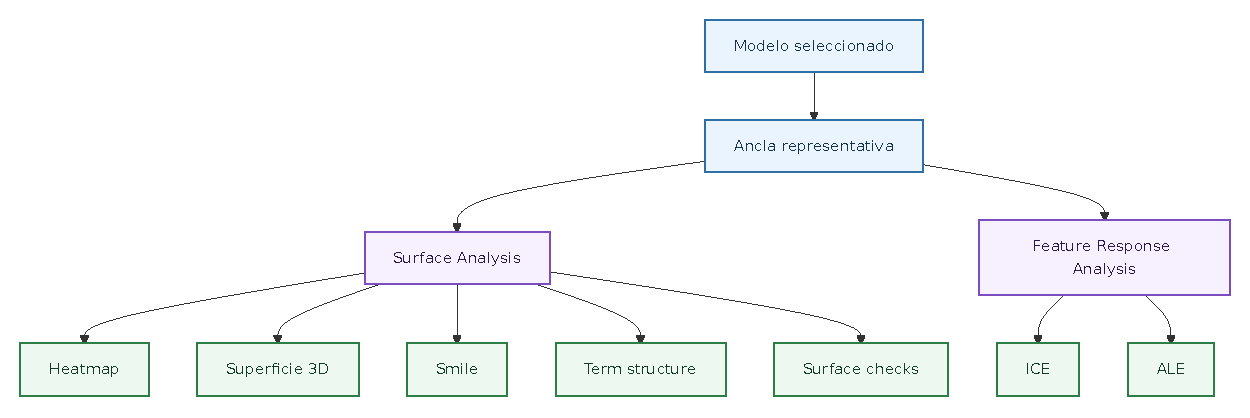
\includegraphics[width=0.92\textwidth,height=0.30\textheight,keepaspectratio]{../doc/mermaid-pdf/dashboard/behaviour-surface/01.pdf}%
\caption{\small Flujo de la pestaña Behaviour And Surface.}
\label{fig:doc-dashboard-behaviour-surface-1}
\end{figure}


\vspace{-0.3cm}
\begin{figure}[!htpb]
\centering
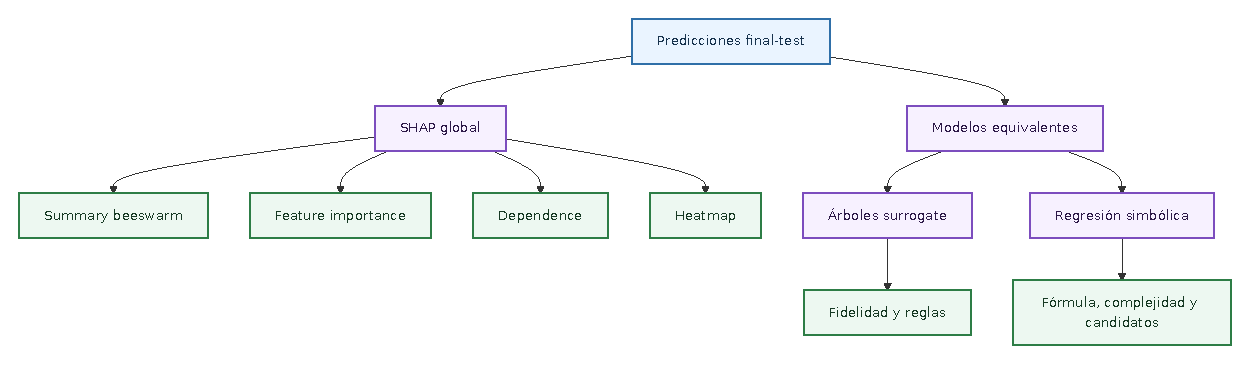
\includegraphics[width=\textwidth,height=0.35\textheight,keepaspectratio]{../doc/mermaid-pdf/dashboard/global-explainability/01.pdf}%
\caption{\small Flujo de la pestaña Global Explainability.}
\label{fig:doc-dashboard-global-explainability-1}
\hfill
\end{figure}

\begin{figure}[h]
\centering
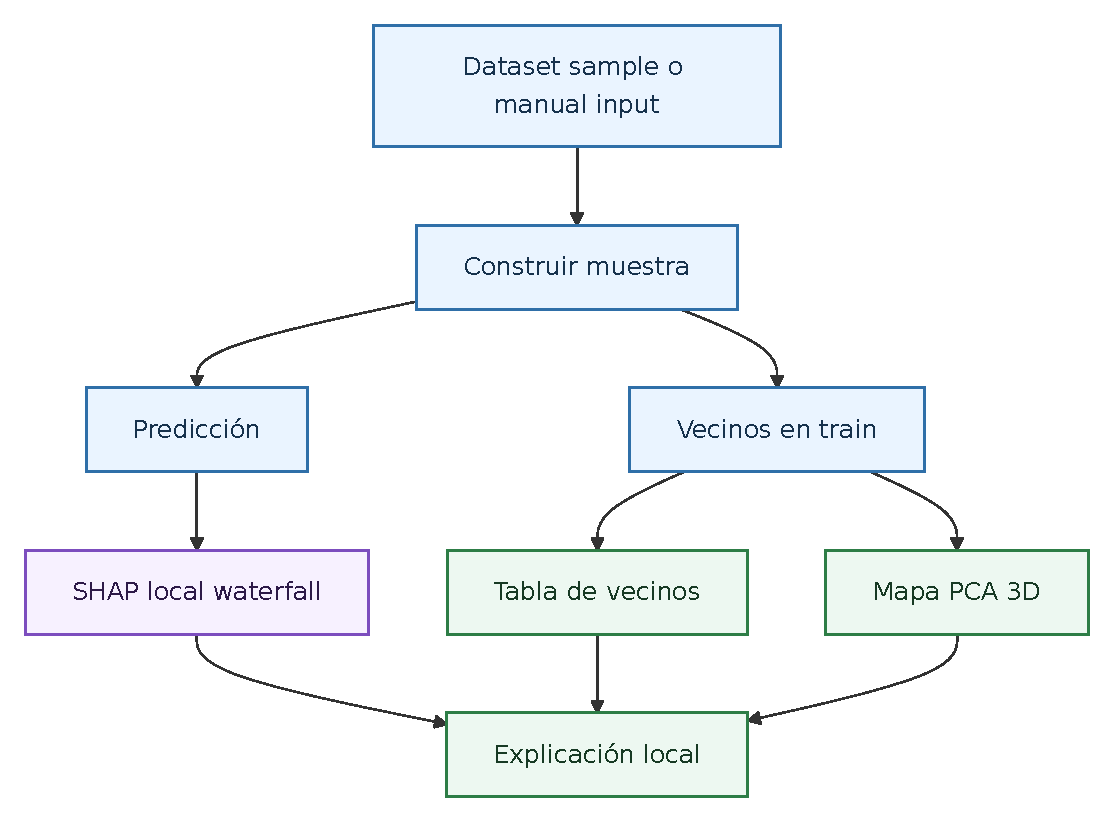
\includegraphics[width=\textwidth,height=0.35\textheight,keepaspectratio]{../doc/mermaid-pdf/dashboard/sample-explainability/01.pdf}%
\caption{\small Flujo de la pestaña Sample Explainability.}
\label{fig:doc-dashboard-sample-explainability-1}
\end{figure}

\vspace{-0.3cm}
\begin{figure}[h]
\centering
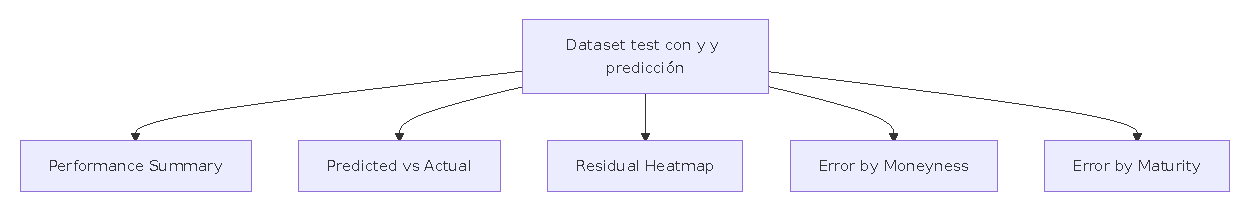
\includegraphics[width=0.92\textwidth,height=0.30\textheight,keepaspectratio]{../doc/mermaid-pdf/dashboard/diagnosis/01.pdf}%
\caption{\small Vistas de diagnóstico del modelo final.}
\label{fig:doc-dashboard-diagnosis-1}
\end{figure}


\vspace{-0.3cm}
\begin{figure}[h]
\centering
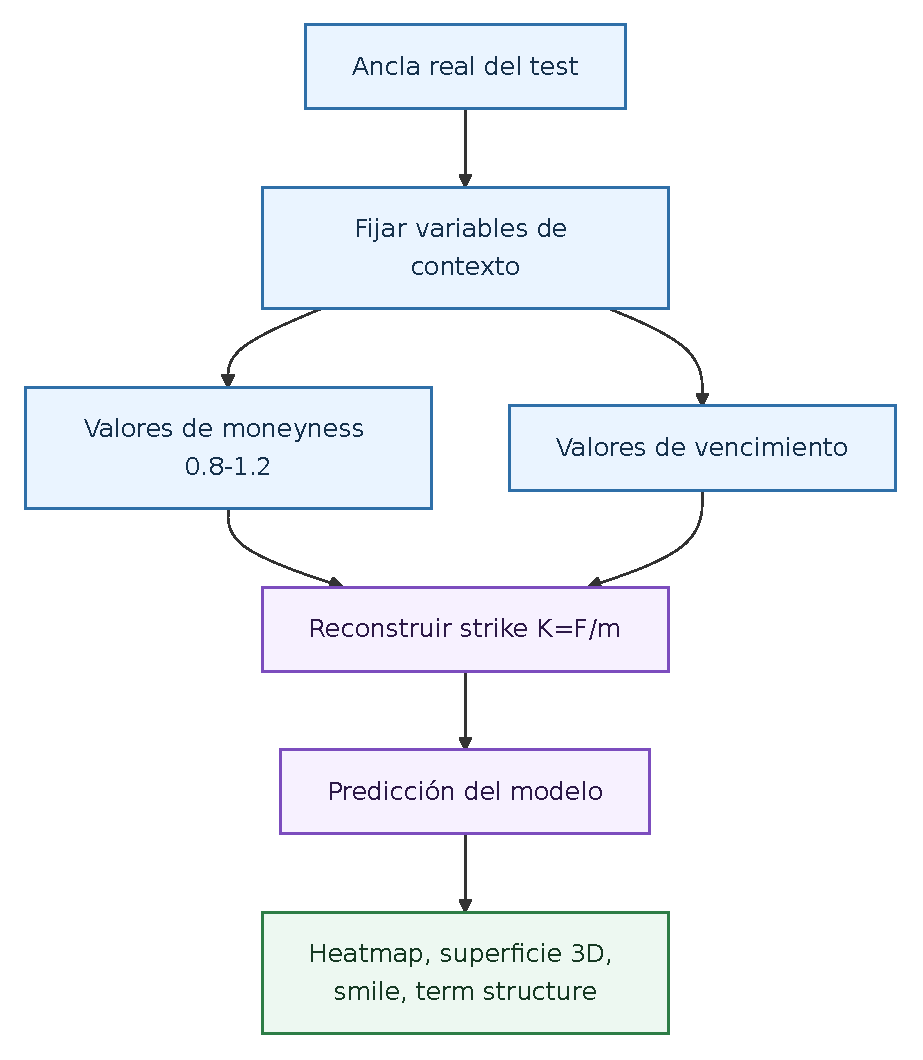
\includegraphics[width=0.80\textwidth,height=0.35\textheight,keepaspectratio]{../doc/mermaid-pdf/dashboard/behaviour/volatility-surfaces/01.pdf}%
\caption{\small Construcción de superficies locales de volatilidad.}
\label{fig:doc-dashboard-behaviour-volatility-surfaces-1}
\end{figure}

\section{API, almacenamiento y cloud}
\label{sec:api-cloud-metodo}

La API se implementa con FastAPI como un servicio \emph{ad hoc} independiente del dashboard. Puede servir cualquier modelo preparado bajo este flujo de entrenamiento, sin depender de la capa visual. En el despliegue objetivo de este trabajo, tanto la API como el dashboard se ejecutan sobre la plataforma Google Cloud Platform (GCP), concretamente en servicios de Cloud Run. El código expone endpoints de salud, predicción y explicabilidad local:

\begin{itemize}[noitemsep]
  \item \texttt{/health}
  \item \texttt{/run\_model/predict/}
  \item \texttt{/run\_model/sample\_explainability/}
\end{itemize}

La petición incluye modelo, tipo de opción, strike, subyacente, tiempo a vencimiento, tipo de interés y, opcionalmente, código de contrato y volatilidad real.

La respuesta de predicción incluye el modelo, la volatilidad estimada y la entrada normalizada. La respuesta de explicabilidad local añade waterfall SHAP, payload de contribuciones, vecinos históricos y distancias. API y dashboard comparten modelos y paquetes autocontenidos de dashboard, lo que reduce el riesgo de explicar una versión distinta de la usada para predecir. La operativa de workflows, automatización y despliegue reproducible que soporta esta separación se desarrolla con más detalle en el apéndice \ref{app:workflow-dev}.



\begin{figure}[!htpb]
\centering
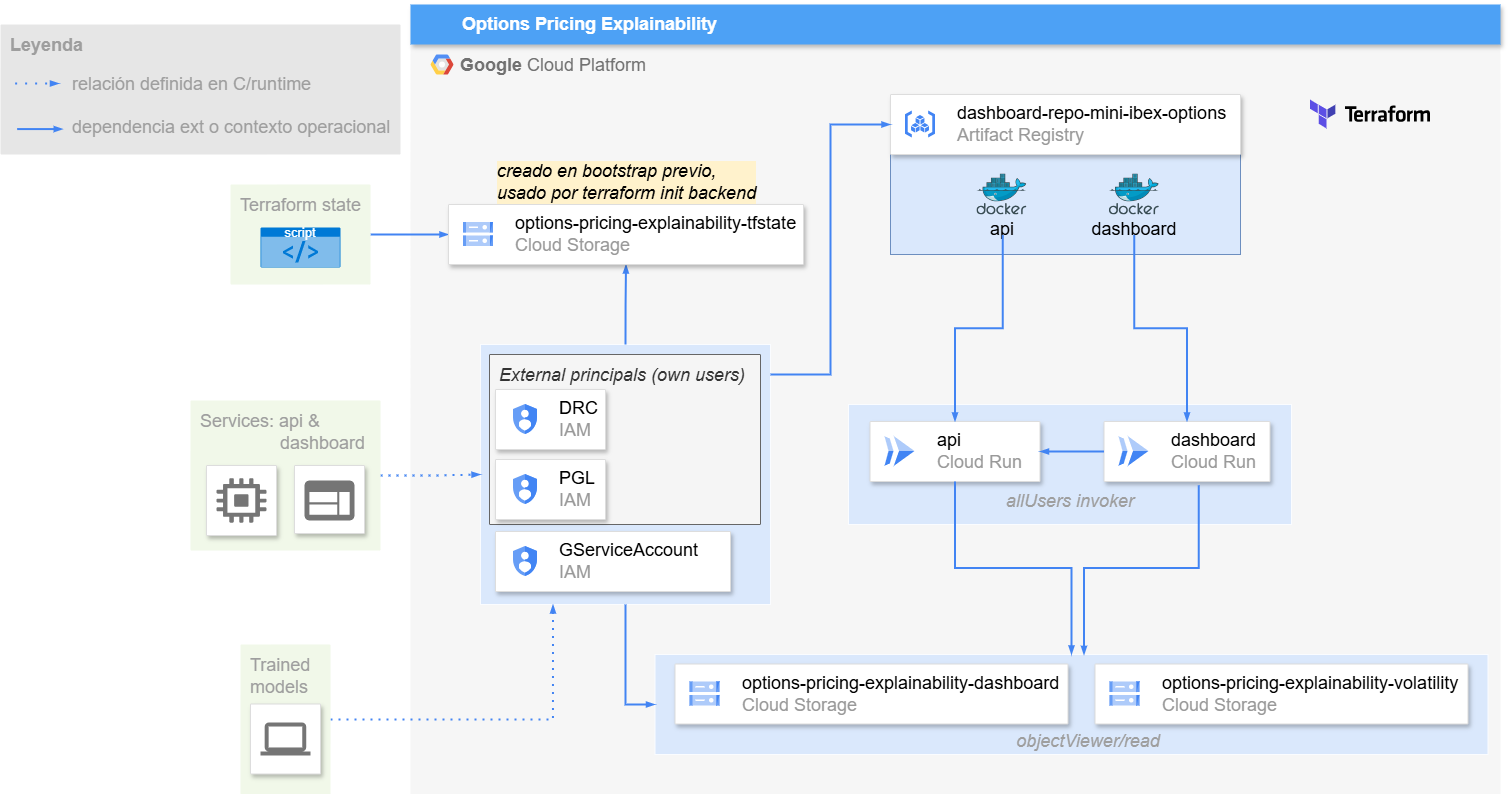
\includegraphics[width=0.96\textwidth,height=0.56\textheight,keepaspectratio]{../imgs/cloud_diagram.drawio.png}%
\caption{\small Arquitectura cloud del sistema: almacenamiento, elementos y servicios de API/dashboard.}
\label{fig:cloud-diagram-drawio}
\end{figure}


El backend de almacenamiento puede ser local o GCP. En el entorno de despliegue del proyecto se utiliza GCP: Cloud Storage para modelos y paquetes de dashboard, Artifact Registry para imágenes de contenedor, Cloud Run para API y dashboard, e IAM para permisos. Terraform define los recursos y permite reproducir la infraestructura. La parte crítica es mantener sincronizados modelo, scaler, metadatos y paquete explicativo; por eso el reentrenamiento final dispara su construcción después de guardar el modelo. La Figura~\ref{fig:cloud-diagram-drawio} resume este esquema de despliegue, dejando explícita la separación entre almacenamiento, artefactos de modelo y servicios desplegados.


\section{reproducibilidad}
\label{sec:reproducibilidad}
El trabajo se ha realizado siguiendo todos los pasos descritos en este documento. De la misma manera, siguiendo todos los pasos descritos en este documento junto con los notebooks de ayuda del repositorio y la  \href{https://epiblasfunds.github.io/options-pricing/}{documentación de github} (\href{https://epiblasfunds.github.io/options-pricing/}{epiblasfunds.github.io/options-pricing/}) es posible reproducir el trabajo si contamos con los datos fuentes necesarios (sino, estos datos pueden ser mockeados).

Lo necesario para reproducir el estudio es llevar a cabo los procesos de:
\begin{enumerate}
    \item Procesado de datos.
    \item Entrenamiento de modelos.
    \item Conversión de modelos entrenados al formato adecuado para presentar en el dashboard.
    \item Tener cuenta de GCP y poder desplegar el dashboard y la API.
\end{enumerate}

Es importante remarcar que aunque la configuración sea la misma es posible que los resultados de entrenamiento varíen un poco y esto provoque métricas, fórmulas de regresión simbólica y árboles de decisión ligeramente distintos.


\section{Arquitectura del repositorio}
\label{sec:arquitectura-repo}

\begin{figure}[h]
\centering
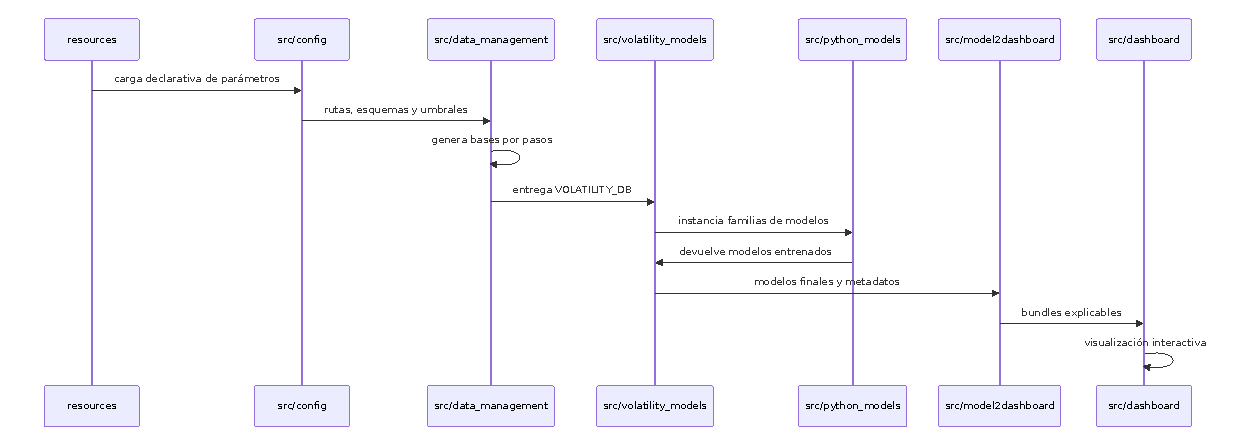
\includegraphics[width=0.92\textwidth,height=0.30\textheight,keepaspectratio]{../doc/mermaid-pdf/repository/index/02.pdf}%
\caption{\small Secuencia de ejecución entre paquetes.}
\label{fig:doc-repository-index-2}
\end{figure}


La arquitectura del repositorio sigue una separación por funcionalidades: cada paquete tiene un cometido identificable y las salidas persistidas pasan de una etapa a otra sin mezclar entrenamiento, explicación y servicio. La Figura~\ref{fig:doc-repository-index-2} muestran la secuencia de ejecución, la cadena de salidas y las dependencias entre paquetes.


\begin{table}[htbp]
\centering
\small
\begin{tabular}{p{0.26\textwidth}p{0.60\textwidth}}
\toprule
Paquete o carpeta & Responsabilidad principal \\
\midrule
\texttt{src/config} & Carga de configuración, rutas absolutas, logging y objetos de configuración por dominio. \\
\texttt{src/enums} & Definición centralizada de columnas, tipos de contrato, tipos de opción y nombres de modelos. \\
\texttt{src/exceptions} & Excepciones de dominio usadas en validaciones de datos y control de errores del ETL. \\
\texttt{src/data\_management} & ETL de datos: loaders, builders, validaciones y utilidades de contrato. \\
\texttt{src/volatility\_models} & Preparación de datos de entrenamiento, splits, k-folds, selección y reentrenamiento. \\
\texttt{src/python\_models} & Abstracciones de familias de modelos y estructuras persistibles de dashboard. \\
\texttt{src/model2dashboard} & Conversión de modelos finales en paquetes explicativos autocontenidos. \\
\texttt{src/dashboard} & Aplicación Dash, servicios, callbacks, gráficos y utilidades de validación. \\
\texttt{src/api} & API FastAPI para predicción y explicabilidad local. \\
\texttt{resources} & Configuración declarativa (datos, modelos y cliente-servidor) consumida por el runtime. \\
\texttt{dockerfiles} & Definiciones de imagen para API, dashboard, LaTeX y utilidades de documentación. \\
\texttt{scripts} & Automatizaciones auxiliares de soporte operativo y generación de artefactos. \\
\texttt{terraform} & Infraestructura cloud reproducible: buckets, registro de imágenes, Cloud Run e IAM. \\
\bottomrule
\end{tabular}
\caption{Arquitectura lógica del repositorio.}
\label{tab:arquitectura-repo}
\end{table}

La Tabla~\ref{tab:arquitectura-repo} muestra que el dashboard no reentrena modelos y la API no reconstruye explicaciones desde cero salvo en casos de explicabilidad local manual. Esta separación reduce el acoplamiento y facilita detectar errores. Si una predicción de API no coincide con la vista del dashboard, el problema puede acotarse a carga del paquete autocontenido, transformación de features o versión de modelo.

Vista así, la arquitectura no es sólo una organización de carpetas. Es una forma de aislar responsabilidades, simplificar depuración y poder justificar cada paso del flujo de principio a fin.

Desde esa misma lógica, la arquitectura se apoya en un flujo de trabajo de ingeniería más próximo al de un proyecto real que al de un experimento ad hoc: ramas de trabajo, commits trazables, validaciones antes de integrar y control explícito de cambios sobre código, configuración, documentación y despliegue. Esa capa metodológica de desarrollo, validación y despliegue se amplía en el apéndice \ref{app:workflow-dev}.

Todos estos paquetes están cubiertos por más del 80\% en cobertura de tests unitarios, haciendo que las funcionalidades sean robustas para futuras evoluciones del código, haciéndolo más escalables. A esta escalabilidad ayuda también el checkeo de formato Flake8. Para obligar a respetar tanto el formato Flake8 como el paso de los tests, se han desarrollado workflows de GitHub para que GitHub actions ejecute en pipelines para comprobar ambas condiciones, tal como se resume de forma específica en el apéndice \ref{app:workflow-dev}.


\section{Riesgos metodológicos y controles}
\label{sec:riesgos}

Los principales riesgos metodológicos se anticipan desde el diseño. 

\begin{enumerate}
    \item Lookahead bias: controlado mediante orden temporal y subyacentes anteriores a la opción.
    \item Data snooping: mitigado separando búsqueda de hiperparámetros, reentrenamiento y evaluación final.
    \item Memorización de contratos: tratado con exclusividad de contratos entre splits.
    \item Extrapolación en zonas poco cubiertas, diagnosticada con vecinos históricos y heatmaps de error. 
    \item Confundir explicabilidad del modelo con verdad de mercado: por ello los surrogates se presentan con métricas de fidelidad y los resultados se contrastan frente a residuales y superficies.
\end{enumerate}
